\section{Data}\label{sec:data}
\setstretch{1.5}

Table \ref{table:stats} presents summary statistics at the baseline year for all the variables used in this analysis: variables related to the EC2/9, fiscal data, health inputs, infant mortality rates, birth outcomes, and control variables. Statistics are presented for the full sample, and for the bottom and top quartile of distribution of municipalities' own resource spending in public health.

\subsection{EC/29 and Fiscal Data}

For evaluating the causal impact of the EC/29 on public spending, we combine public spending data from the Brazilian Finance System (FINBRA)\footnote{All spending data is presented in 2010 R\$. We used the General Price Index (IGP) to correct values}, which covers the period of 1998 to 2010, with data from the Brazilian National System of Public Health Budget (Datasus/SIOPS)\footnote{SIOPS was created right after the EC/29 to monitor revenues and expenditure in the provision of health care at the state and municipal levels, and to monitor compliance with the EC/29.} available from 2000 onward. FINBRA provides data on total public spending, spending by type, and spending by a few aggregated categories, such as Health and Sanitation, Education and Culture, etc, and SIOPS provides data on total health spending, health spending from own resources, health spending from intergovernmental transfers, spending by type, and the share of own resources spent in health.  Additionally, we also gather data on total public revenues and revenues by source (tax or intergovernmental transfers) from FINBRA.


Figure \ref{fig:5} displays the spatial variation in the share of own resources spent in health. Municipalities below the EC/29 are represented with colors in the red scale, while municipalities above the target are represented with the blue scale. The map shows significant differences in the share of own resources spent in health within the same state, providing the identifying variation of this study as we include state fixed-effects in our main specification. 

\begin{figure}[h!]
\begin{center}
    \caption{EC/29 Compliance Geographic Variation}
    \scalebox{0.7}{
    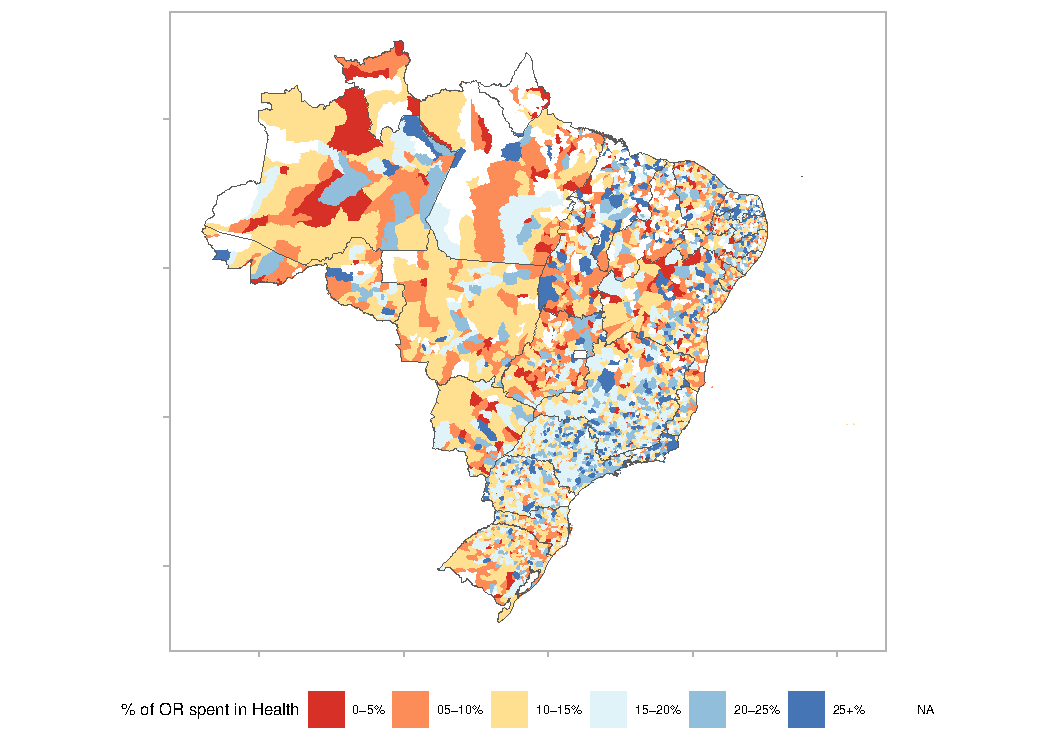
\includegraphics{plots/ec29_map.pdf}
    \label{fig:5}
    }
\end{center}
\end{figure}

\subsection{Infant Mortality and Birth Outcomes}

We use micro-data from Brazilian National System of Mortality Records (Datasus/SIM) and from the Brazilian National System of Birth Records (Datasus/SINASC) to construct Infant Mortality Rates. These micro-data allow us to construct Infant Mortality Rates by timing of death, and for the main causes of death. Moreover, following \cite{alfradique2009internaccoes} classification we are able to construct mortality rates amenable and non-amenable to primary care.

The SINASC micro-data records all births in Brazil and provides detailed information on these births, such as Apgar 1 and 5, birth weight and gestation weeks.

\subsection{Health Inputs}

There is no data available on municipalities' supply of public health infrastructure for the period of this analysis. However, we are able to indirectly construct proxies for public health infrastructure using the micro-data from the National System of Information on Ambulatory Care (Datasus/SIA). This database records every ambulatorial procedure funded by SUS, with information on the type and complexity of the procedure, the health professional responsible, and the corresponding health facility register number. Using this data we are able to calculate the number of health facilities with ambulatory service in a municipality, as well as the number of facilities with ambulatory services classified by the type of service and professional responsible for the service \footnote{We are able to construct these variables only for the period of 1998 to 2007, as changes in the SIA classification of ambulatorial procedures changes in 2008.}. Variables on the access to healthcare were constructed using data from the Brazilian National System of Information on Primary Care (Datasus/SIAB) and from SINASC. Primary care coverage at the intensive and extensive margin data comes from SIAB and data on the access to health services from SINASC. Lastly, we use SIA micro-data to build data on ambulatory production.

\subsection{Controls}

Our control variables can be classified into two different categories: socioeconomic controls and fiscal controls. The first, comes from the Census of 2000. The later, from FINBRA dataset. We use as fiscal controls the average health spending per capita in the bordering municipalities\footnote{cite Mattos article} and a dummy that indicates whether a municipalities spend more than 60\% of its revenue with personnel, non complying with the Fiscal Responsibility Law of 2000.

